\documentclass[tikz, border=4pt]{standalone}
\usepackage{tikz}
\usetikzlibrary{automata, arrows.meta}
\begin{document}
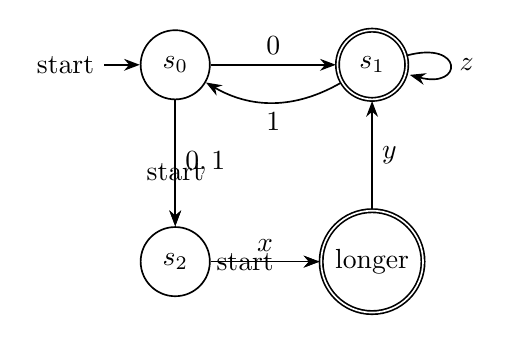
\begin{tikzpicture}[x=1cm, y=1cm]
  \begin{scope}[shift={(1.77,-0.47)}, ->, >=Stealth, auto, node distance=2.5cm, semithick]
    \node[state, initial, initial text=start] (a) {$s_0$};
    \node[state, accepting] (b) [right of=a] {$s_1$};
    \node[state, initial above] (c) [below of=a] {$s_2$};
    \node[state, initial left, accepting] (d) [below of=b] {longer};
    \path (a) edge node {$0$} (b)
          (b) edge [bend left] node {$1$} (a)
          (a) edge node {$0,1$} (c)
          (c) edge node {$x$} (d)
          (d) edge node[swap] {$y$} (b)
          (b) edge [loop right] node {$z$} ();
  \end{scope}
\end{tikzpicture}
\end{document}
